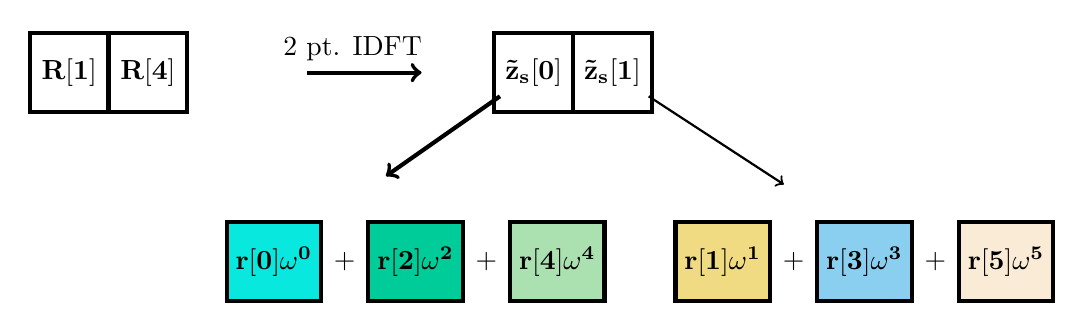
\begin{tikzpicture}

\definecolor{brightturquoise}{rgb}{0.03, 0.91, 0.87}
\definecolor{buff}{rgb}{0.94, 0.86, 0.51}
\definecolor{caribbeangreen}{rgb}{0.0, 0.8, 0.6}
\definecolor{celadon}{rgb}{0.67, 0.88, 0.69}
\definecolor{darktangerine}{rgb}{1.0, 0.66, 0.07}
\definecolor{darkviolet}{rgb}{0.58, 0.0, 0.83}
\definecolor{deepskyblue}{rgb}{0.0, 0.75, 1.0}
\definecolor{amber(sae/ece)}{rgb}{1.0, 0.49, 0.0}
\definecolor{antiquewhite}{rgb}{0.98, 0.92, 0.84}
\definecolor{applegreen}{rgb}{0.55, 0.71, 0.0}
\definecolor{babyblue}{rgb}{0.54, 0.81, 0.94}



% x_{s} (down-sample by 2)
\draw[thick,line  width =1.5pt]  (4.4,0) rectangle (5.4,-1);
\draw[thick,line  width =1.5pt]  (5.4,0) rectangle (6.4,-1);

\node at (4.9,-0.5) {$\bf R[1]$};
\node at (5.9,-0.5) {$\bf R[4]$};


% DFT arrow
\node (v1) at (7.8,-0.5) {};
\node (v2) at (9.5,-0.5) {};
\draw[thick, ->,line  width =1.5pt]  (v1) edge (v2);
\node at (8.5,-0.2) {2 pt.  IDFT};

% X_{s} (DFT of x_{s})
\draw[thick,line  width =1.5pt]  (10.3,0) rectangle (11.3,-1);
\draw[thick,line  width =1.5pt]  (11.3,0) rectangle (12.3,-1);

\node (v3) at (10.8,-0.5) {$\bf \tilde{z}_{s}[0]$};
\node (v5) at (11.8,-0.5) {$\bf \tilde{z}_{s}[1]$};


\node (v4) at (8.8,-1.9) {};
\node (v6) at (14.1,-2) {};

\draw[thick,->,line  width =1.5pt]  (v3) edge (v4);
\draw[thick,->]  (v5) edge (v6);
\draw[thick,fill=brightturquoise,line  width =1.5pt]  (6.9,-2.4) rectangle (8.1,-3.4);
\draw[thick,fill=babyblue,line  width =1.5pt]  (14.4,-2.4) rectangle (15.6,-3.4);
\draw[thick,fill=buff,line  width =1.5pt]  (12.6,-2.4) rectangle (13.8,-3.4);
\draw[thick,fill=celadon,line  width =1.5pt]  (10.5,-2.4) rectangle (11.7,-3.4);
\draw[thick,fill=caribbeangreen,line  width =1.5pt]  (8.7,-2.4) rectangle (9.9,-3.4);
\draw[thick,fill=antiquewhite,line  width =1.5pt]  (16.2,-2.4) rectangle (17.4,-3.4);


\node at (7.5,-2.9) {$\bf r[0] \omega^{0}$};
\node at (15,-2.9) {$\bf r[3] \omega^{3}$};
\node at (8.4,-2.9) {$\mathbf{+}$};

\node at (13.2,-2.9) {$\bf r[1] \omega^{1}$};
\node at (11.1,-2.9) {$\bf r[4] \omega^{4}$};
\node at (10.2,-2.9) {$\mathbf{+}$};

\node at (9.3,-2.9) {$\bf r[2] \omega^{2}$};
\node at (16.8,-2.9) {$\bf r[5] \omega^{5}$};
\node at (14.1,-2.9) {$\mathbf{+}$};
\node at (15.9,-2.9) {$\mathbf{+}$};
\end{tikzpicture} 